% Conversion avec : convert -density 300 -flatten img.pdf img.png
\documentclass{standalone}
\usepackage{xcolor,pgf,tikz,tkz-tab,pgfplots,xfp}
\pgfplotsset{compat=1.15}
\usetikzlibrary{arrows,backgrounds,calc}
\begin{document}
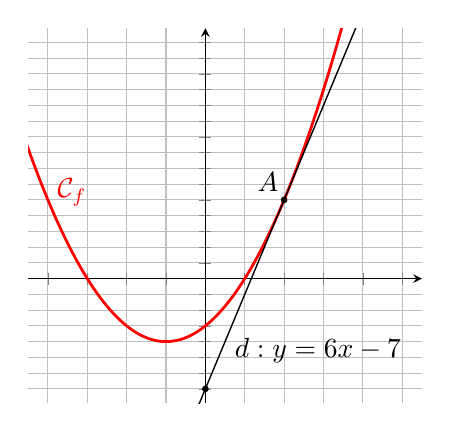
\begin{tikzpicture}
	\begin{axis}[x=0.5cm,y=0.2cm,axis lines=middle,ymajorgrids=true,xmajorgrids=true,xmin=-4.5,xmax=5.5,ymin=-7.9,ymax=15.9,xtick={-8.0,-7.0,...,6.0},ytick={-8.0,-7.0,...,17.0},yticklabel=\empty,xticklabel=\empty]
		\draw[line width=1.0pt,color=red,smooth,samples=100,domain=-7:4] plot(\x,{(\x)^(2.0)+2*(\x)-3});
		\draw[line width=0.5pt,color=black,smooth,samples=10,domain=-7:4] plot(\x,{6*(\x)-7});
		\draw [fill=black] (0,-7) circle (1pt);
		\draw [fill=black] (2,5) circle (1pt);
		\draw [color=red] (-4,4) node[anchor=south west] {$\mathcal{C}_f$};
		\draw [color=black] (.5,-6) node[anchor=south west] {$d:y=6x-7$};
		\draw [color=black] (2.1,4.9) node[anchor=south east] {$A$};
	\end{axis}
\end{tikzpicture}
\end{document}
